%! TEX root = ../dissertation_gurecky.tex

\section{5x5 Results}

All axial crud results for the 5x5 model are shown in figures \ref{fig:montageaxialbmasssm} and \ref{fig:montageaxialcmasssm}.  The axial distributions are shown at a simulated time of 300 days. Pin-integrated crud results plotted as a function of time are provided in figures \ref{fig:montagetimebmasssm} and \ref{fig:montagetimecmasssm}.

\begin{landscape}
\begin{figure}[H]
    \centering
    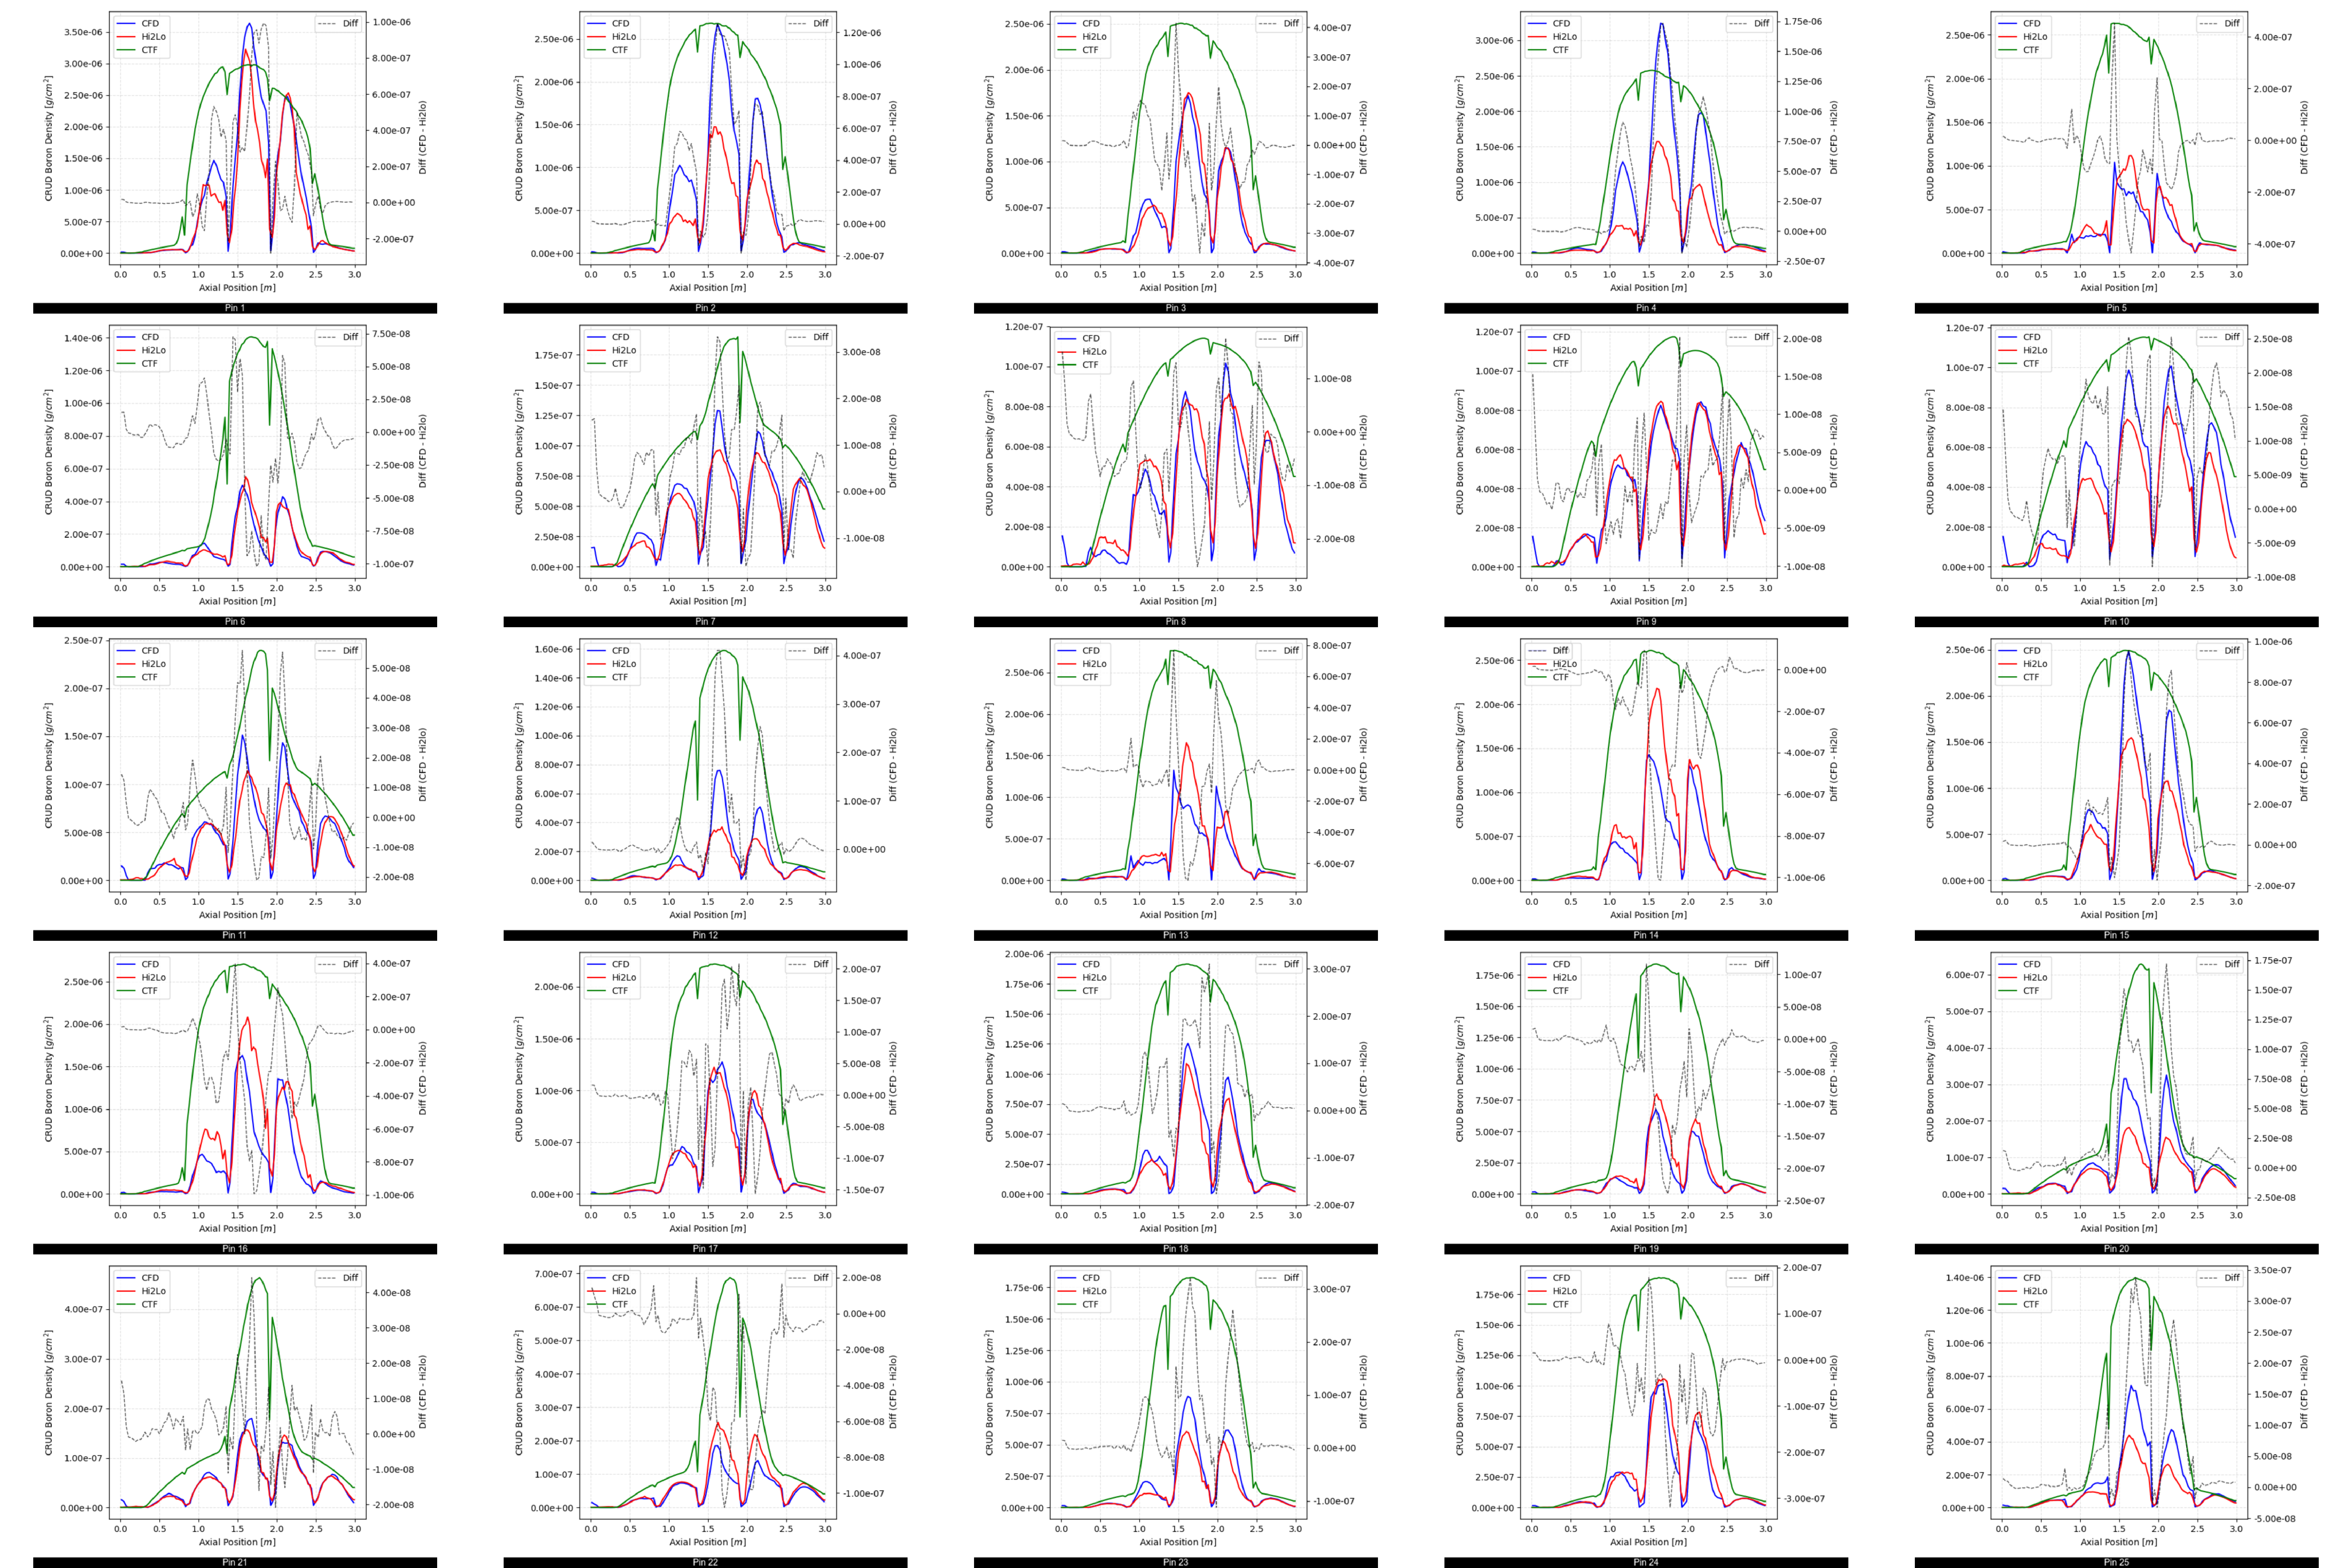
\includegraphics[width=.9\linewidth]{figs/5x5/imp/montage_axial_bmass_sm}
    \caption{5x5 axial crud boron mass results at 300 days.}
    \label{fig:montageaxialbmasssm}
\end{figure}
\begin{figure}[H]
    \centering
    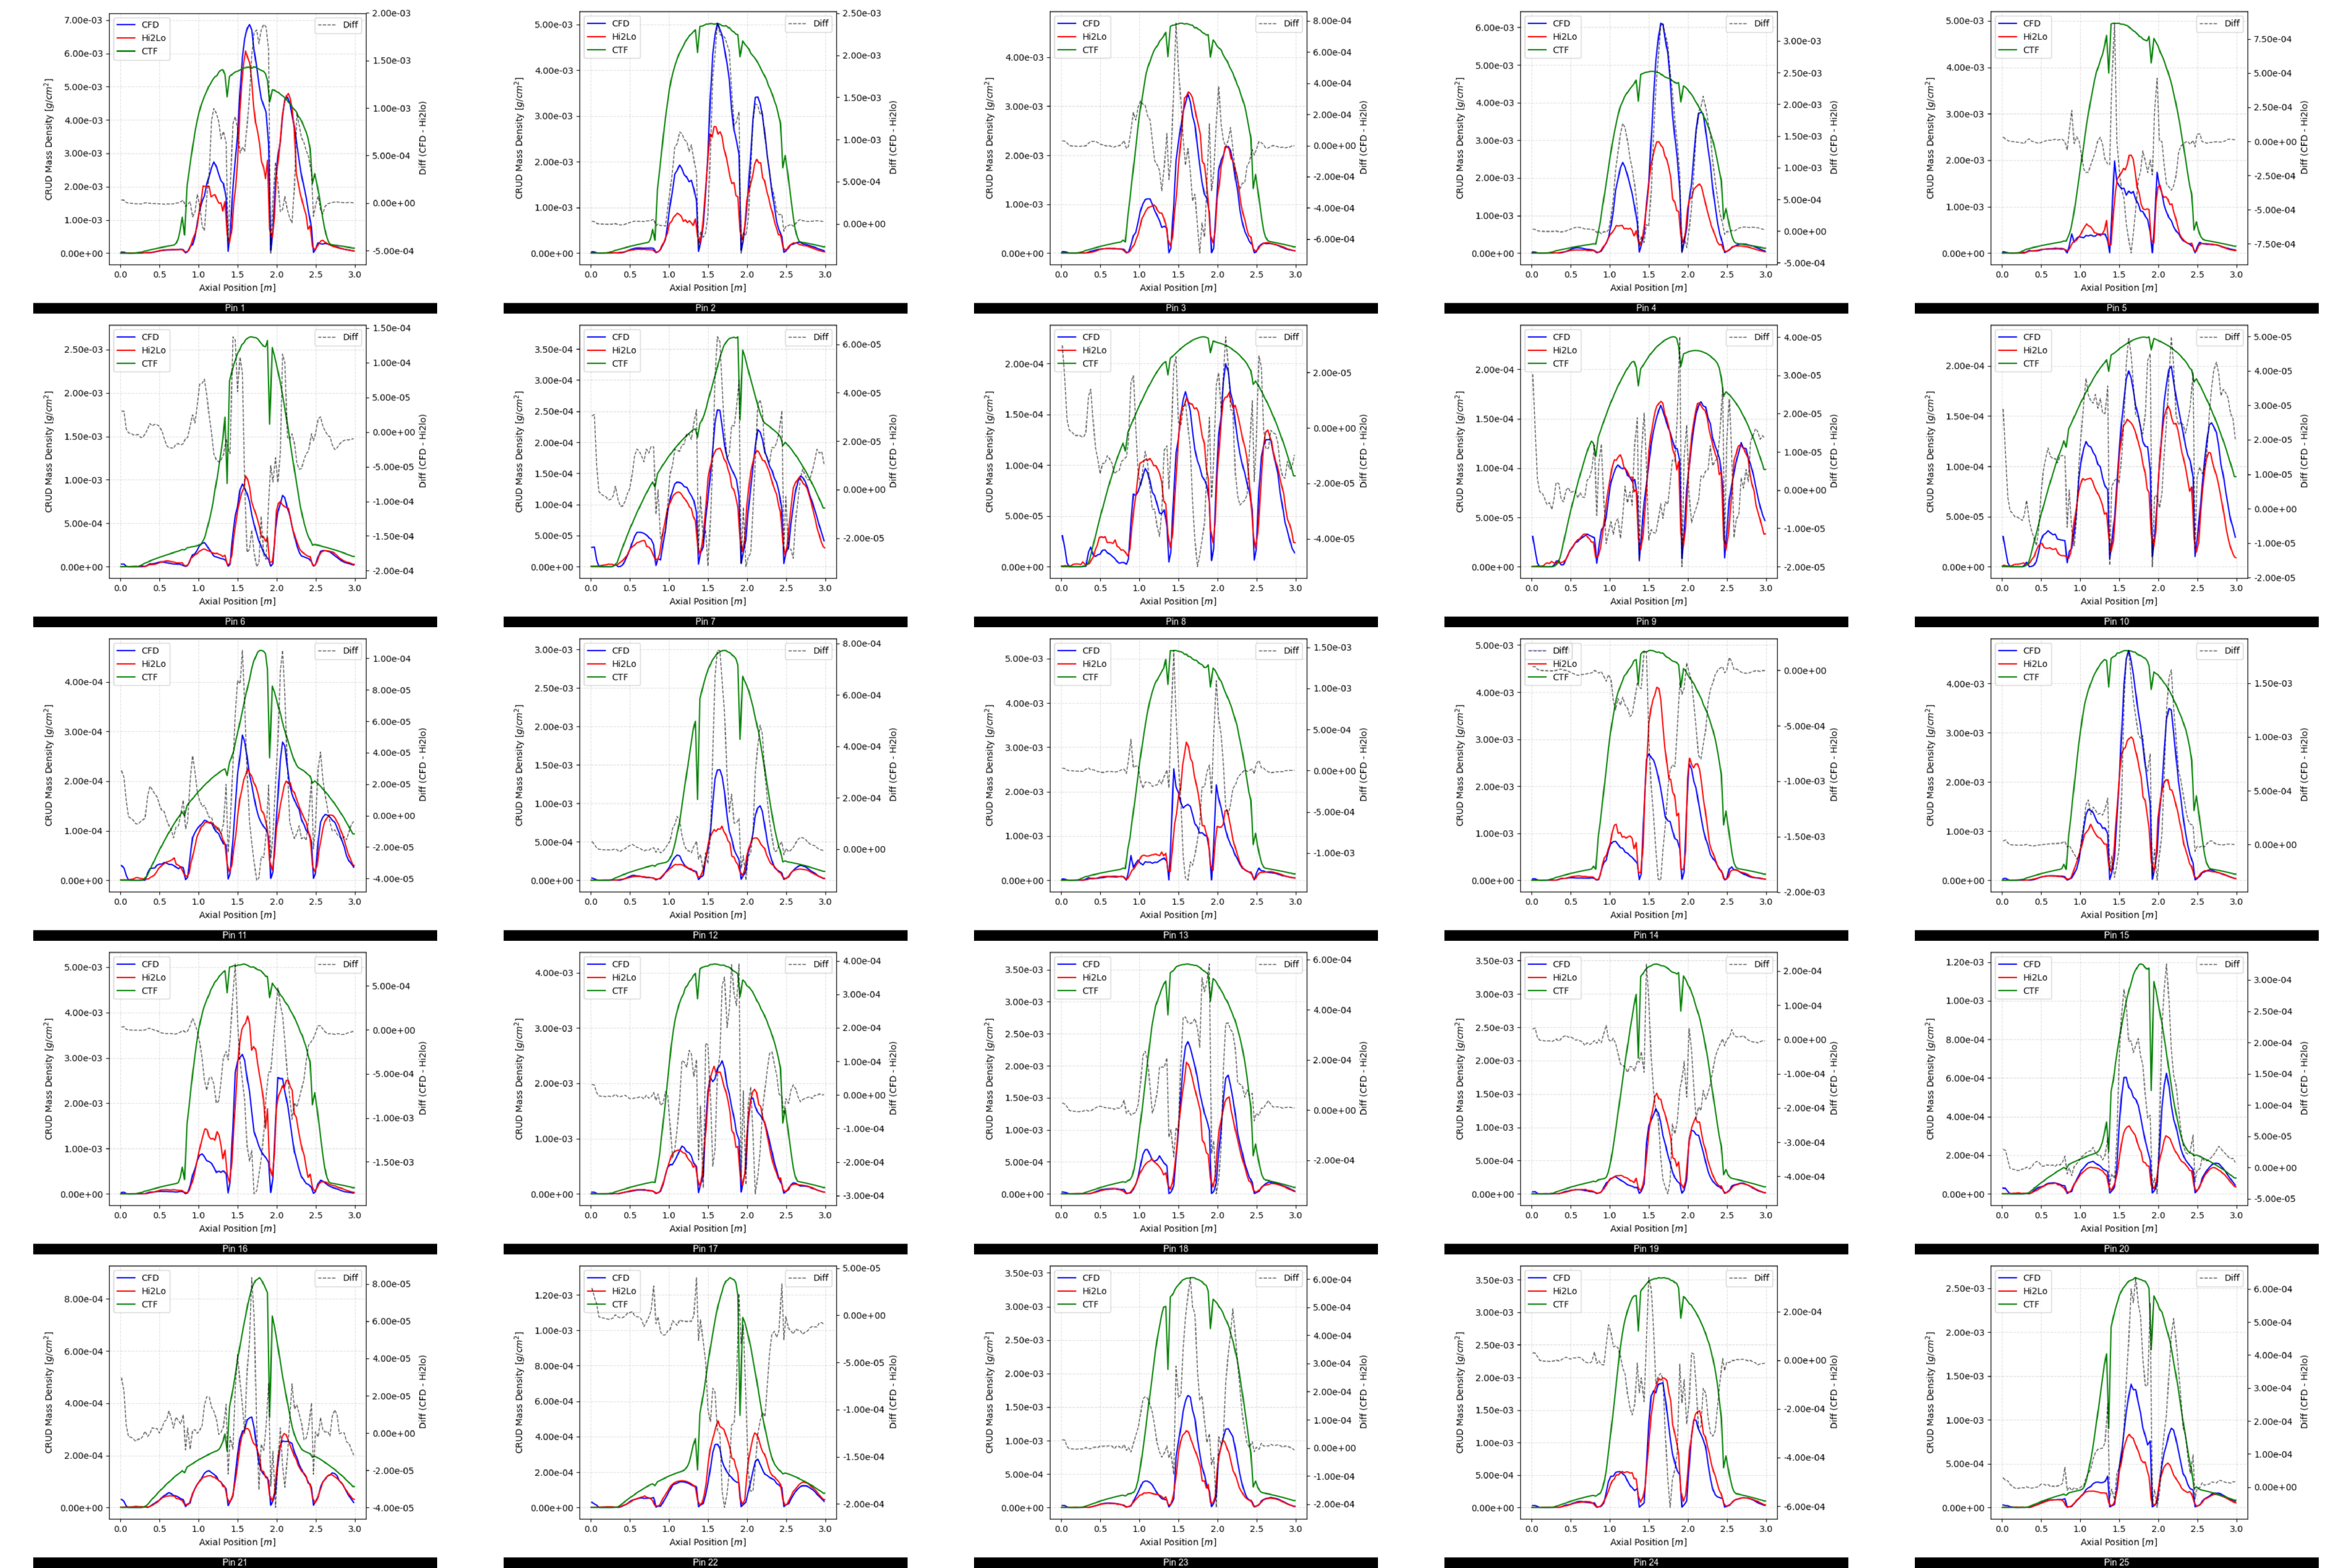
\includegraphics[width=.9\linewidth]{figs/5x5/imp/montage_axial_cmass_sm}
    \caption{5x5 axial crud mass results at 300 days.}
    \label{fig:montageaxialcmasssm}
\end{figure}

\begin{figure}[H]
    \centering
    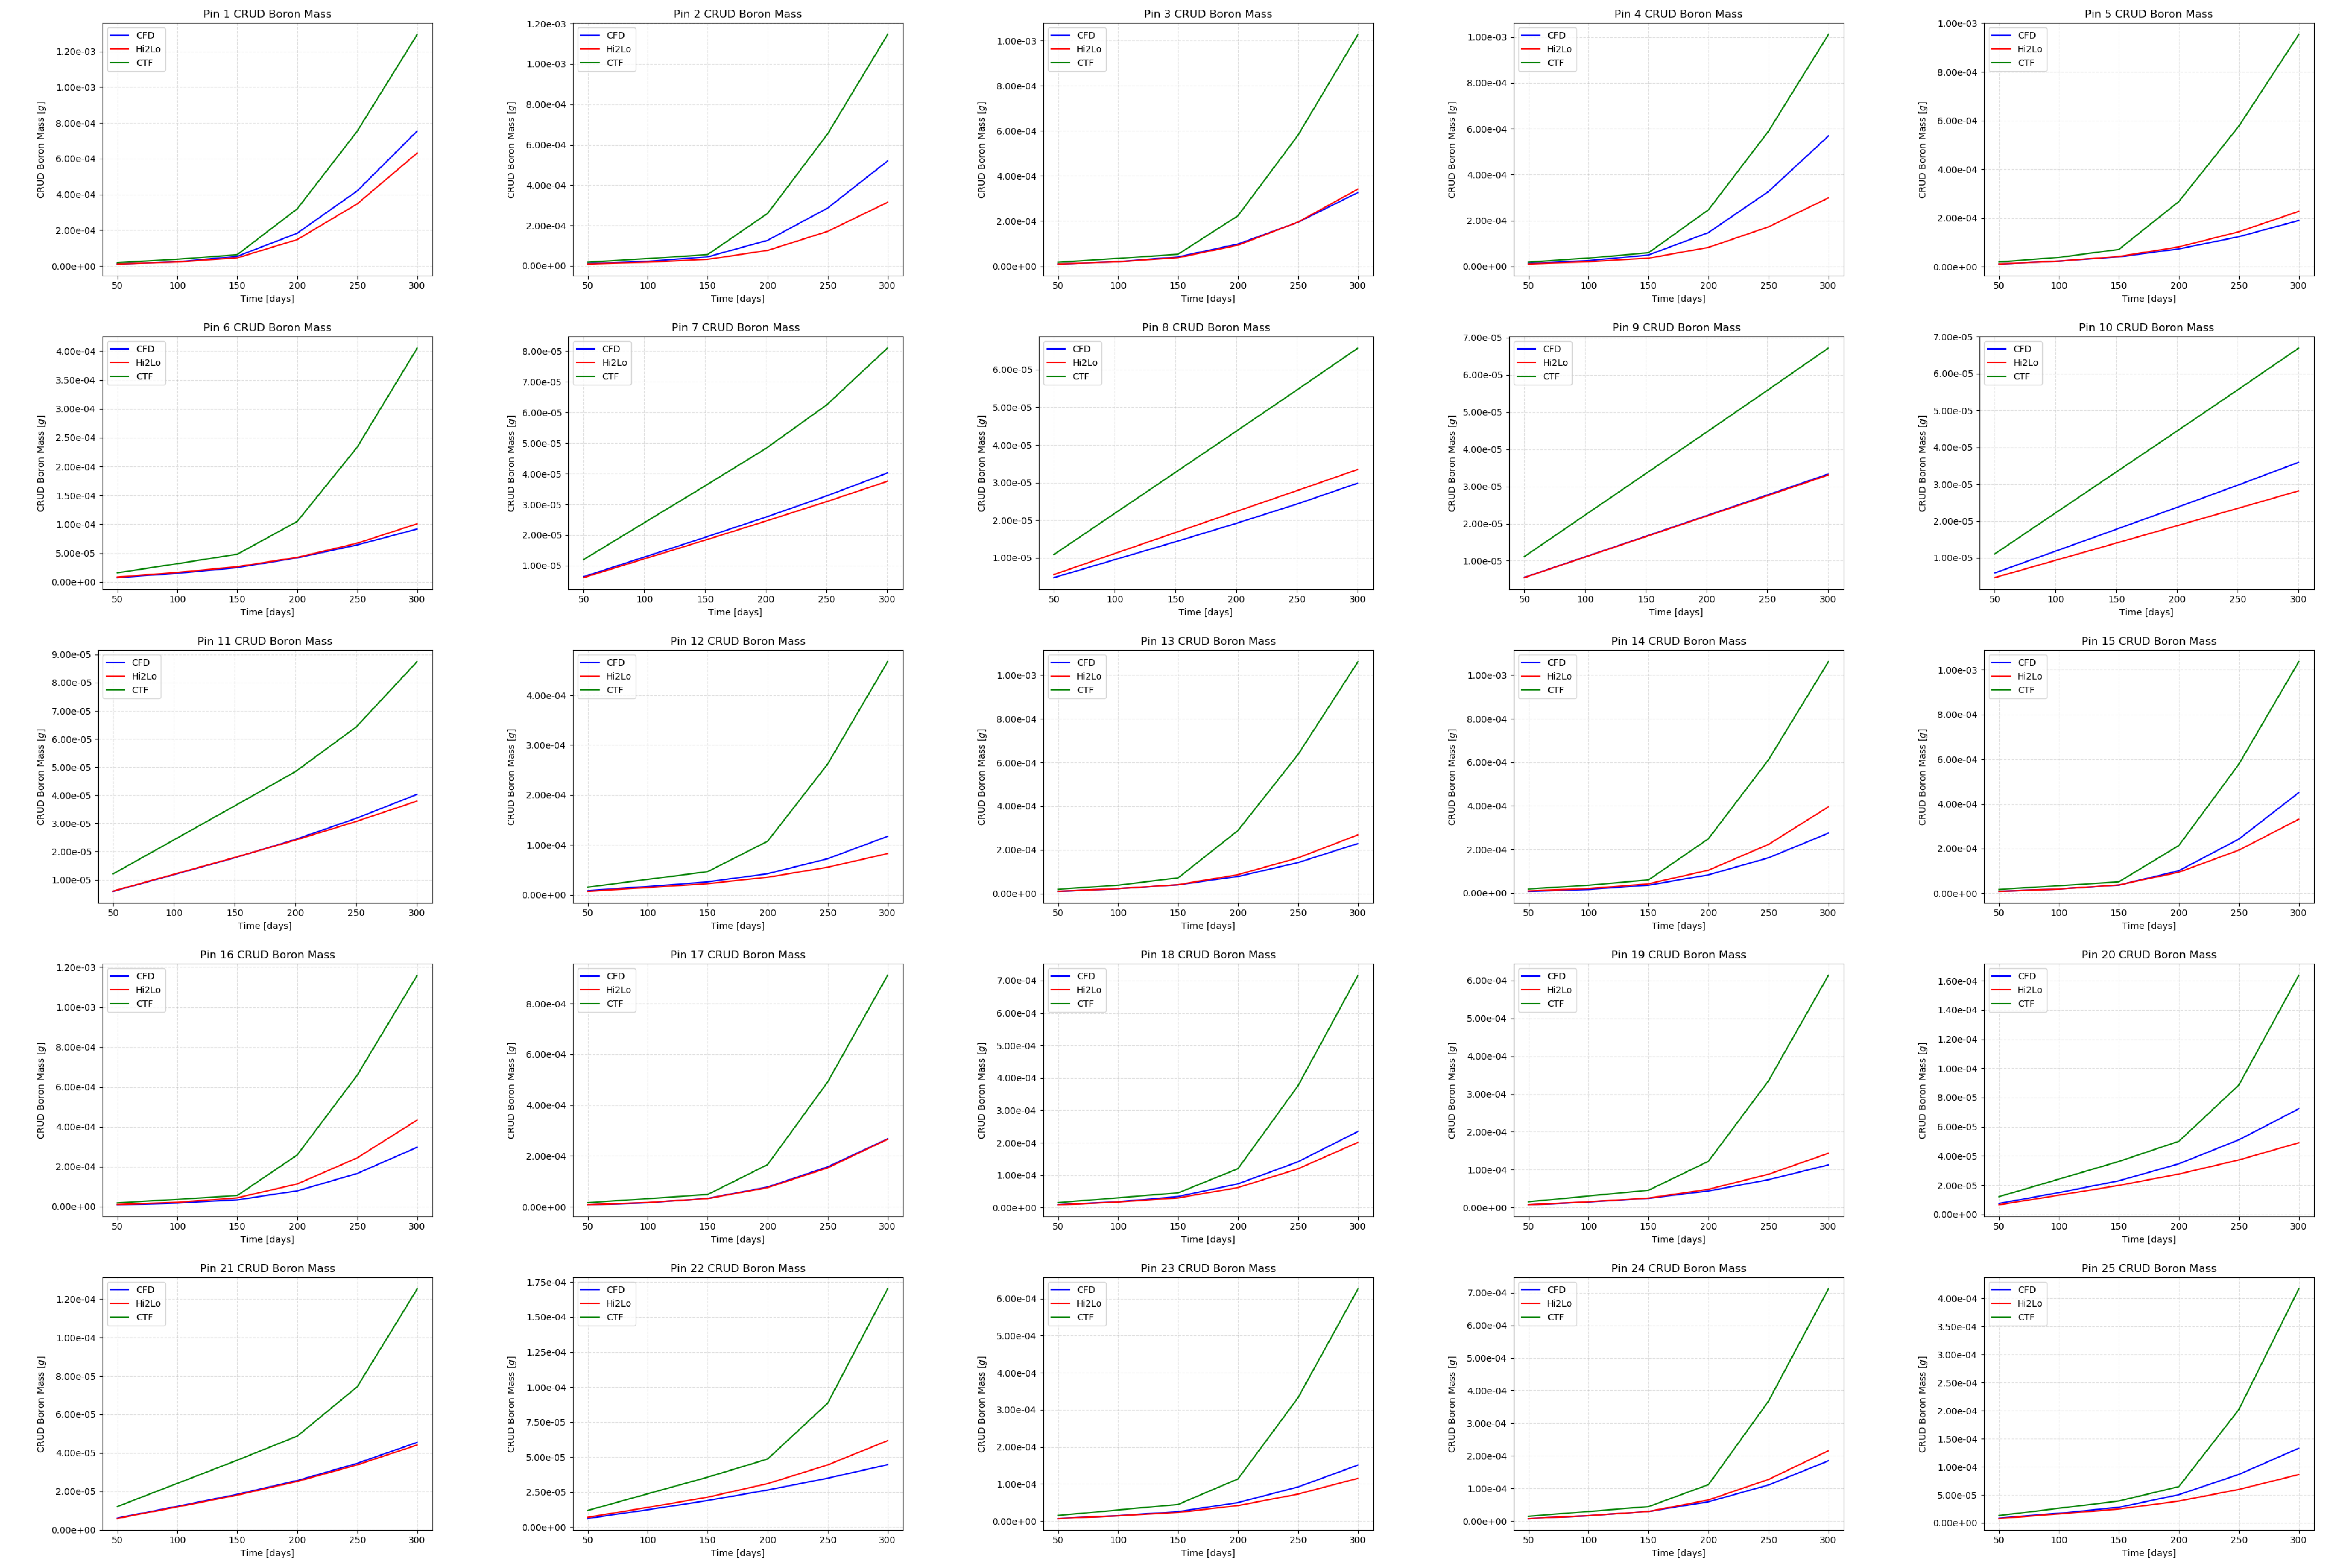
\includegraphics[width=0.9\linewidth]{figs/5x5/imp/montage_time_bmass_sm}
    \caption{5x5 rod integrated crud boron mass vs time.}
    \label{fig:montagetimebmasssm}
\end{figure}


\begin{figure}[H]
    \centering
    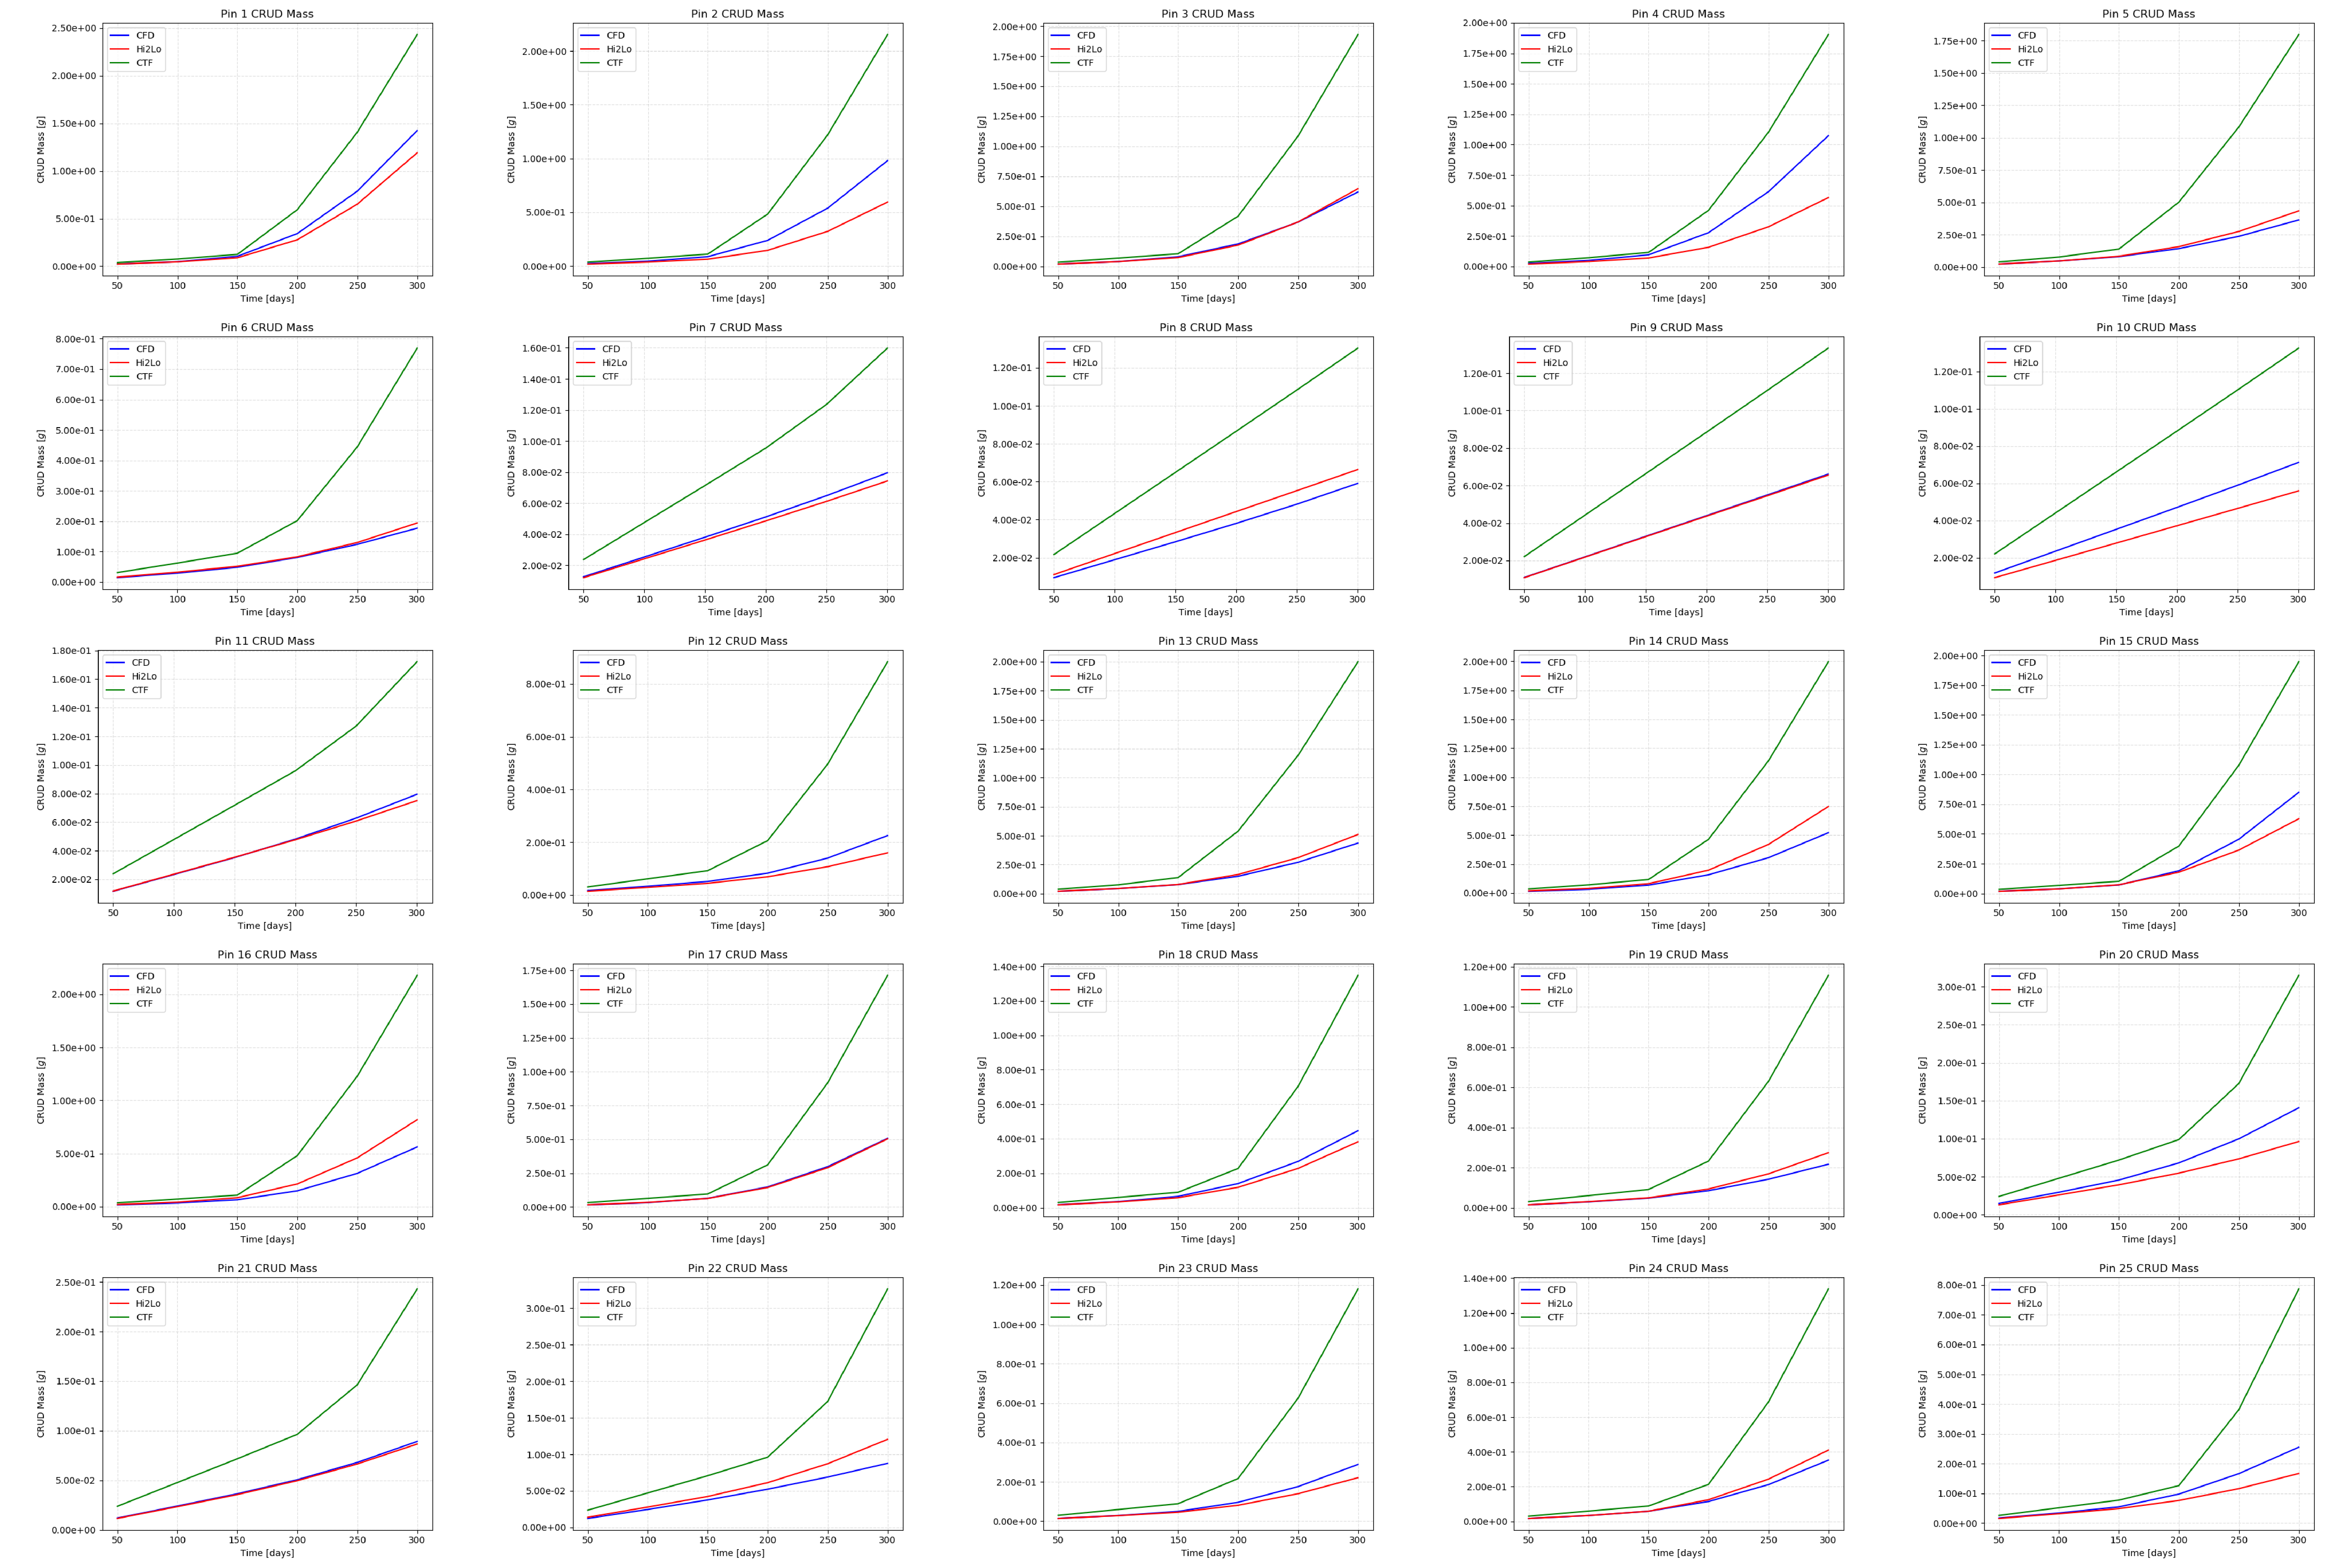
\includegraphics[width=0.9\linewidth]{figs/5x5/imp/montage_time_cmass_sm}
    \caption{5x5 rod integrated crud mass vs time.}
    \label{fig:montagetimecmasssm}
\end{figure}

\end{landscape}
